\section{Engineering Background}
% REVISIT: what to put here?
% research on possible architectures
% hardware of FPGA
% speed of memory
% launch registers
% PLLs
% HLS vs Verilog?
% LFSR

\subsection{Target}
The design of the verification system is the major engineering challenge of this
project.
In order to stress the DUT, the verification system must perform at a much
higher frequency than the expected frequency of the DUT.
Assuming the DUT is to run at 300MHz, to fully explore the effect of
overclocking, the testbench must be able to run at double the frequency or
higher.
This gives a target frequency of 800MHz.
Assuming data width of 32-bits, the target data transfer rate is then 
This required data transfer rate is estimated to be 25.6Gbps.

\subsection{Data Transfer Rate}
% REVISIT: possible to find exact bandwidth of the bridge?
As the test is to be run on the HPS, the HPS-FPGA bridge will be the
immediate bottleneck if the test data is to flow from HPS to FPGA.
While HPS is able to easily generate test data,
there is a large amount of overhead as data crosses from one architecture
to another.
This overhead exists in terms of both a lowered bandwidth and a high delay.
Thus, it would not be sensible for HPS to send out data during run-time.

% --- using SDRAM
Another thought may be to first populate the off-chip DDR SDRAM on FPGA
side, then feed the data from there to the DUT during test.
This is already much faster than passing the data from HPS.
The 1GB, 32-bits wide DDR3 on FPGA side is rated at 400MHz.
With double rate transfer, this would gives a maximum transfer rate of 25.6Gbps.

While using the off-chip RAM may theoretically achieve the targets,
it still has its disadvantages.
First, the process of filling up the memory and then using them for the tests
takes time.
This means the test would be broken up into bursts with time in between for
checking the results and filling up with new data.
The complexity of the SDRAM interface also requires a SDRAM controller to be
used to manage SDRAM refresh cycles, address multiplexing and interface timing.
These all adds up to a significant access latency.
While this could be overcame with burst accesses and piplined accesses,
it would further complicate the SDRAM controller.
While this controller is provided by Altera~\cite{Altera3}, it is consumes
a non-negligible amount of the limited FPGA resources, while adding
unnecessary complexity to the design.
Customising the controller to fit this project may also be time-consuming.

% --- on-chip memory
The on-chip memory is much faster and simpler to handle.
This memory is implemented on the FPGA itself, and thus there is no external
connections for access to this memory.
It has the highest possible throughput, with the lowest possible latency
in an FPGA-based system.
The memory transactions can also be piplined, giving one transaction per
clock cycle.
With an on-chip FIFO accessed in dual-port mode, the write at one end and the
reads at the other end can happen simultaneously.
This effective doubling of the bandwidth is useful as tests are prepared
and fed into the DUT, or when test results are collected and fed to a checker.

On-chip memory is not without its drawbacks.
It is volatile and very limited in capacity.
While the off-chip can have its storage reaching 1GB, that of the on-chip
memory could only reach a few MB~\cite{Altera2}.
Volatility is not exactly of concern in this project, but its small capacity
means not much test data can be held before it needs more fed in.

Looking at the options listed above, with a way of generating test data at
run-time on the FPGA, using on-chip memory would be the most sensible option.


\subsection{Clock Domains}
Another concern in the system design is of the different clock domains that
must exist on the FPGA.
At a minimum, there needs to be two clock domains, one surrounds the DUT and
another supports the rest of the control logic around the DUT.

These clock frequencies can be generated and distributed with PLLs provided as
an IP in the Quartus software~\cite{Altera4}.

\subsection{Testbench Architecture}
\newcommand{\mx}[1]{\mathbf{\bm{#1}}} % Matrix command
\newcommand{\vc}[1]{\mathbf{\bm{#1}}} % Vector command

% We need layers to draw the block diagram
\pgfdeclarelayer{background}
\pgfdeclarelayer{foreground}
\pgfsetlayers{background,main,foreground}

% Define a few styles and constants
\tikzstyle{sensor}=[draw, fill=blue!20, text width=5em, 
    text centered, minimum height=2.5em]
\tikzstyle{ann} = [above, text width=5em]
\tikzstyle{naveqs} = [sensor, text width=6em, fill=red!20, 
    minimum height=12em, rounded corners]
\def\blockdist{2.3}
\def\edgedist{2.5}

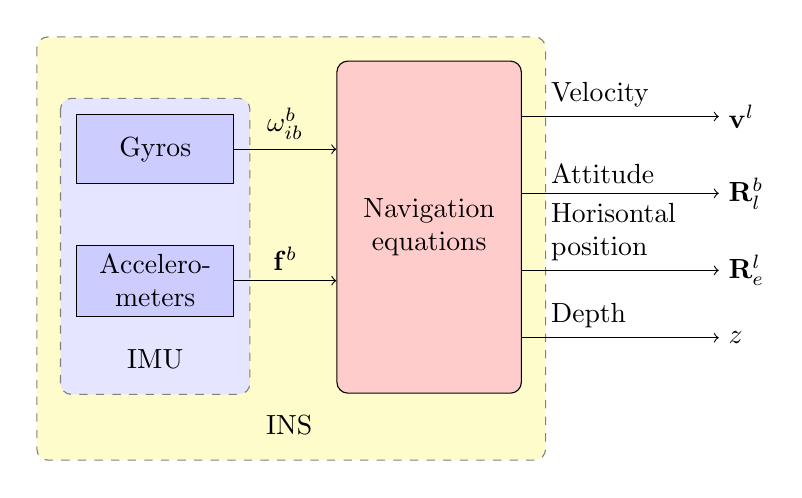
\begin{tikzpicture}
    \node (naveq) [naveqs] {Navigation equations};
    % Note the use of \path instead of \node at ... below. 
    \path (naveq.140)+(-\blockdist,0) node (gyros) [sensor] {Gyros};
    \path (naveq.-150)+(-\blockdist,0) node (accel) [sensor] {Accelero-meters};
    
    % Unfortunately we cant use the convenient \path (fromnode) -- (tonode) 
    % syntax here. This is because TikZ draws the path from the node centers
    % and clip the path at the node boundaries. We want horizontal lines, but
    % the sensor and naveq blocks aren't aligned horizontally. Instead we use
    % the line intersection syntax |- to calculate the correct coordinate
    \path [draw, ->] (gyros) -- node [above] {$\vc{\omega}_{ib}^b$} 
        (naveq.west |- gyros) ;
    % We could simply have written (gyros) .. (naveq.140). However, it's
    % best to avoid hard coding coordinates
    \path [draw, ->] (accel) -- node [above] {$\vc{f}^b$} 
        (naveq.west |- accel);
    \node (IMU) [below of=accel] {IMU};
    \path (naveq.south west)+(-0.6,-0.4) node (INS) {INS};
    \draw [->] (naveq.50) -- node [ann] {Velocity } + (\edgedist,0) 
        node[right] {$\vc{v}^l$};
    \draw [->] (naveq.20) -- node [ann] {Attitude} + (\edgedist,0) 
        node[right] { $\mx{R}_l^b$};
    \draw [->] (naveq.-25) -- node [ann] {Horisontal position} + (\edgedist,0)
        node [right] {$\mx{R}_e^l$};
    \draw [->] (naveq.-50) -- node [ann] {Depth} + (\edgedist,0) 
        node[right] {$z$};
    
    % Now it's time to draw the colored IMU and INS rectangles.
    % To draw them behind the blocks we use pgf layers. This way we  
    % can use the above block coordinates to place the backgrounds   
    \begin{pgfonlayer}{background}
        % Compute a few helper coordinates
        \path (gyros.west |- naveq.north)+(-0.5,0.3) node (a) {};
        \path (INS.south -| naveq.east)+(+0.3,-0.2) node (b) {};
        \path[fill=yellow!20,rounded corners, draw=black!50, dashed]
            (a) rectangle (b);
        \path (gyros.north west)+(-0.2,0.2) node (a) {};
        \path (IMU.south -| gyros.east)+(+0.2,-0.2) node (b) {};
        \path[fill=blue!10,rounded corners, draw=black!50, dashed]
            (a) rectangle (b);
    \end{pgfonlayer}
\end{tikzpicture}


% use this after different clock speeds are introduced
Chapter 4 of Shi's paper~\cite{Shi1} provides a similar structure for this
verification system.